\section*{Problem 3: Rot-Schwarz Bäume} 

Ein rot-schwarz Baum ist ein binärer Suchbaum, den wir auf die folgende Weise erweitern: Jeder Knoten und jeder leere Teilbaum erhält eine Farbe (rot oder schwarz), so dass die folgenden Regeln gelten: (i) die Wurzel ist schwarz; (ii) die leeren Teilbäume sind schwarz; (iii) die Kinder eines roten Knoten sind schwarz; und (iv) die schwarze Tiefe aller leeren Teilbäume ist gleich, d.h., für alle leeren Teilbäume ist die Anzahl der schwarzen Knoten auf dem Pfad von der Wurzel zum jeweiligen Teilbaum gleich.\\

\noindent
\textbf{a)} Zeichnen Sie drei Beispiele für rot-schwarz Bäume und erklären Sie, warum diese jeweils die Regeln für einen rot-schwarz Baum erfüllen. 


\begin{enumerate}

\item \textbf{Beispiel}


\begin{tikzpicture}[scale=0.5,
  level 1/.style={sibling distance=80mm},
  level 2/.style={sibling distance=60mm},
  level 3/.style={sibling distance=40mm},
  level 4/.style={sibling distance=20mm}]
\node{$50^{3}$}
	child{node{$10^{0}$}
		child{node{$\Box^{-1}$}}
		child{node{$\Box^{-1}$}}}
	child{node{\textcolor{red}{$100^{2}$}}
		child{node{$75^{0}$}
			child{node{$\Box^{-1}$}}
			child{node{$\Box^{-1}$}}}
		child{node{$150^{1}$}
			child{node{\textcolor{red}{$125^{0}$}}
				child{node{$\Box^{-1}$}}
				child{node{$\Box^{-1}$}}}
			child{node{\textcolor{red}{$175^{0}$}}
				child{node{$\Box^{-1}$}}
				child{node{$\Box^{-1}$}}}}};
\end{tikzpicture}


\begin{itemize}
	\item[(i)] Wurzel ist schwarz
	\item[(ii)] alle leeren Teilbäume sind schwarz
	\item[(iii)] Kinderknoten von \textcolor{red}{100} sind schwarz(75,150)
	\item[(iv)]:
	\begin{itemize}
		\item linker Teilbaum(10): von der Wurzel bis zu den leeren Teilbäumen haben wir $1$ schwarzen Knoten (10)
		\item rechter Teilbaum(100-150-175): von der Wurzel bis zu den leeren Teilbaum haben wir $1$ schwarzen Knoten (150)
	\end{itemize}
\end{itemize}

\textbf{\item Beispiel}

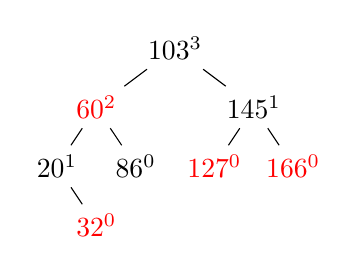
\begin{tikzpicture}[scale=0.5,
  level 1/.style={sibling distance=40mm},
  level 2/.style={sibling distance=20mm},
  level 3/.style={sibling distance=20mm},
  level 4/.style={sibling distance=20mm}]
\node{$103^{3}$}
	child{node{$\textcolor{red}{60^{2}}$}
		child{node{$\textcolor{black}{20^{1}}$}
			child[missing]
			child{node{$\textcolor{red}{32^{0}}$}}}
		child{node{$\textcolor{black}{86^{0}}$}}}
	child{node{\textcolor{black}{$145^{1}$}}
		child{node{$\textcolor{red}{127^{0}}$}}
		child{node{$\textcolor{red}{166^{0}}$}}};
\end{tikzpicture}

\begin{itemize}
	\item[(i)] Wurzel ist schwarz
	\item[(ii)] alle leeren Teilbäume sind schwarz (aus Platzgründen weggelassen)
	\item[(iii)] Kinderknoten von \textcolor{red}{60} sind schwarz(20,86)
	\item[(iv)]:
	\begin{itemize}
		\item linker Teilbaum(60-20-32): von der Wurzel bis zu den leeren Teilbäumen haben wir $1$ schwarzen Knoten (20)
		\item linker Teilbaum(60-86): von der Wurzel bis zu den leeren Teilbäumen haben wir $1$ schwarzen Knoten (86)
		\item rechter Teilbaum(145-127): von der Wurzel bis zu den leeren Teilbaum haben wir $1$ schwarzen Knoten (145)
		\item rechter Teilbaum(145-166): von der Wurzel bis zu den leeren Teilbaum haben wir $1$ schwarzen Knoten (145)
	\end{itemize}
\end{itemize}

\textbf{\item Beispiel (Falsch)}

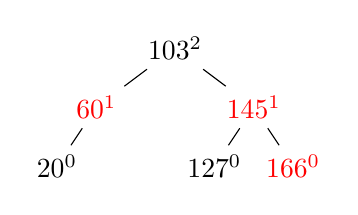
\begin{tikzpicture}[scale=0.5,
  level 1/.style={sibling distance=40mm},
  level 2/.style={sibling distance=20mm},
  level 3/.style={sibling distance=20mm},
  level 4/.style={sibling distance=20mm}]
\node{$103^{2}$}
	child{node{$\textcolor{red}{60^{1}}$}
		child{node{$\textcolor{black}{20^{0}}$}}
		child[missing]}
	child{node{\textcolor{red}{$145^{1}$}}
		child{node{$\textcolor{black}{127^{0}}$}}
		child{node{$\textcolor{red}{166^{0}}$}}};
\end{tikzpicture}

\begin{itemize}
	\item[(i)] Wurzel ist schwarz
	\item[(ii)] alle leeren Teilbäume sind schwarz (aus Platzgründen weggelassen)
	\item[(iii)] Kinderknoten von (\textcolor{red}{60,145}) ist schwarz(20,127)
	\item[(iii)] Kinderknoten von \textcolor{red}{145} ist rot(166) - Verletzung der Schwarz-Rot-Baum-Eigenschaft!
\end{itemize}

$\Rightarrow$ Die ist aufgrund der Verletzung von (iii) kein gültiger Schwarz-Rot-Baum! Siehe \textbf{3.1} für die Korrigierte Variante.

\item[\textbf{3.1}]\textbf{Beispiel (Richtig)}

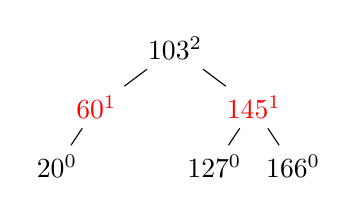
\begin{tikzpicture}[scale=0.5,
  level 1/.style={sibling distance=40mm},
  level 2/.style={sibling distance=20mm},
  level 3/.style={sibling distance=20mm},
  level 4/.style={sibling distance=20mm}]
\node{$103^{2}$}
	child{node{$\textcolor{red}{60^{1}}$}
		child{node{$\textcolor{black}{20^{0}}$}}
		child[missing]}
	child{node{\textcolor{red}{$145^{1}$}}
		child{node{$\textcolor{black}{127^{0}}$}}
		child{node{$\textcolor{black}{166^{0}}$}}};
\end{tikzpicture}

\begin{itemize}
	\item[(i)] Wurzel ist schwarz
	\item[(ii)] alle leeren Teilbäume sind schwarz (aus Platzgründen weggelassen)
	\item[(iii)] Kinderknoten von (\textcolor{red}{60,145}) ist schwarz(20,127,166)
	\item[(iv)]:
	\begin{itemize}
		\item linker Teilbaum(60-20): von der Wurzel bis zu den leeren Teilbäumen haben wir $1$ schwarzen Knoten (20)
		\item rechter Teilbaum(145-127): von der Wurzel bis zu den leeren Teilbaum haben wir $1$ schwarzen Knoten (127)
		\item rechter Teilbaum(145-166): von der Wurzel bis zu den leeren Teilbaum haben wir $1$ schwarzen Knoten (166)
	\end{itemize}
\end{itemize}
\end{enumerate}


\newpage
\noindent
\textbf{b)} Sei $T$ ein rot-schwarz Baum, und sei $s$ die schwarze Tiefe der leeren Teilbäume. Zeigen Sie, dass $T$ mindestens $2s-1 - 1$ schwarze Knoten besitzt. Was folgt daraus über die Mindestanzahl von Knoten in einem rot-schwarz Baum mit Höhe $h$? Folgern Sie: ein rot-schwarz Baum mit $n$ Knoten hat Höhe $O(log n)$.\\


\textbf{Annahme:} Anzahl der Schwarzen Knoten in einem red-black-tree: $2^{s-1}-1$, dabei gelten (i)-(iv) aus der Aufgabenstellung.\\
\textbf{base-case:} red-black-tree, $s=2$ (leerer Baum mit Wurzel):

\begin{verbatim}
  r 		 | depth: 1 (root is black)
 / \
bn bn 	| depth: 2 (black null leaves)
\end{verbatim}
nach (i) gilt: $Num_{blackNodes}=1$\\
$Num_{blackNodes}=2^{2-1}-1=2^{0}-1=2-1=1$\\

Die Annahme gilt im Base-case, Voraussetzung: die Formel $2^{s-1}-1$ gilt für red-black-trees mit $s=k$ schwarzer Tiefe.\\

\textbf{I.S} red-black-tree, mit $s=k+1:$\\
nach (i)-(iv) gilt:
\begin{itemize}
	\item Die Wurzel ist Schwarz
	\item Jeder Teilbaum der Wurzel hat eine schwarze Tiefe von $k$
	\item Jeder Teilbaum hat nach Annahme mindestens $2^{k-1}-1$ schwarze Knoten
\end{itemize}
$Num_{blackNodes} \geq 1+2(2^{k-1}-1)=1+2^{1} * 2^{k-1} -2 = 2^k -1$ $| k = s-1$\\
$Num_{blackNode} \geq 2^{s-1}-1$\\

Die Formel aus der Annahme gilt auch im Induktionsschritt. \\

Laut Definition ist die schwarze Tiefe die Anzahl der Schwarzen Knoten von der Wurzel, bis einem Blatt, wobei Blätter ebenfalls schwarz sind.\\
d.h für die Anzahl schwarzer Knoten im einem red-black-tree gilt: $Num_{blackNode} \geq h/2$, wobei $h$ die Höhe des gesamten Baumes ist.\\
daraus folgt: $Num_{blackNodes} \leq 2^{h/2 -1}-1$ | nach $h$ umformen:\\
$h \geq 2(log(Num_{blackNodes} +1)+1)$ $\rightarrow$ $h \geq 2(log(n +1)+1)$ die Dominate Komplexitätsklasse ist $O((log n))$ \\
daher gilt für die Höhe eines red-black-tree $h<= O(log(n))$\\

\noindent
Quellen:\\
\url{https://medium.com/data-science/understanding-time-complexity-with-python-examples-2bda6e8158a7}
\url{https://www.geeksforgeeks.org/introduction-to-red-black-tree/#interesting-points-about-redblack-tree}





















